% Options for packages loaded elsewhere
\PassOptionsToPackage{unicode}{hyperref}
\PassOptionsToPackage{hyphens}{url}
%
\documentclass[
]{article}
\usepackage{amsmath,amssymb}
\usepackage{iftex}
\ifPDFTeX
  \usepackage[T1]{fontenc}
  \usepackage[utf8]{inputenc}
  \usepackage{textcomp} % provide euro and other symbols
\else % if luatex or xetex
  \usepackage{unicode-math} % this also loads fontspec
  \defaultfontfeatures{Scale=MatchLowercase}
  \defaultfontfeatures[\rmfamily]{Ligatures=TeX,Scale=1}
\fi
\usepackage{lmodern}
\ifPDFTeX\else
  % xetex/luatex font selection
\fi
% Use upquote if available, for straight quotes in verbatim environments
\IfFileExists{upquote.sty}{\usepackage{upquote}}{}
\IfFileExists{microtype.sty}{% use microtype if available
  \usepackage[]{microtype}
  \UseMicrotypeSet[protrusion]{basicmath} % disable protrusion for tt fonts
}{}
\makeatletter
\@ifundefined{KOMAClassName}{% if non-KOMA class
  \IfFileExists{parskip.sty}{%
    \usepackage{parskip}
  }{% else
    \setlength{\parindent}{0pt}
    \setlength{\parskip}{6pt plus 2pt minus 1pt}}
}{% if KOMA class
  \KOMAoptions{parskip=half}}
\makeatother
\usepackage{xcolor}
\usepackage[margin=1in]{geometry}
\usepackage{longtable,booktabs,array}
\usepackage{calc} % for calculating minipage widths
% Correct order of tables after \paragraph or \subparagraph
\usepackage{etoolbox}
\makeatletter
\patchcmd\longtable{\par}{\if@noskipsec\mbox{}\fi\par}{}{}
\makeatother
% Allow footnotes in longtable head/foot
\IfFileExists{footnotehyper.sty}{\usepackage{footnotehyper}}{\usepackage{footnote}}
\makesavenoteenv{longtable}
\usepackage{graphicx}
\makeatletter
\def\maxwidth{\ifdim\Gin@nat@width>\linewidth\linewidth\else\Gin@nat@width\fi}
\def\maxheight{\ifdim\Gin@nat@height>\textheight\textheight\else\Gin@nat@height\fi}
\makeatother
% Scale images if necessary, so that they will not overflow the page
% margins by default, and it is still possible to overwrite the defaults
% using explicit options in \includegraphics[width, height, ...]{}
\setkeys{Gin}{width=\maxwidth,height=\maxheight,keepaspectratio}
% Set default figure placement to htbp
\makeatletter
\def\fps@figure{htbp}
\makeatother
\setlength{\emergencystretch}{3em} % prevent overfull lines
\providecommand{\tightlist}{%
  \setlength{\itemsep}{0pt}\setlength{\parskip}{0pt}}
\setcounter{secnumdepth}{-\maxdimen} % remove section numbering
\usepackage{fancyhdr}
\pagestyle{fancy}
\fancyhf{}
\rfoot{\thepage}
\usepackage{booktabs}
\usepackage{longtable}
\usepackage{array}
\usepackage{multirow}
\usepackage{wrapfig}
\usepackage{float}
\usepackage{colortbl}
\usepackage{pdflscape}
\usepackage{tabu}
\usepackage{threeparttable}
\usepackage{threeparttablex}
\usepackage[normalem]{ulem}
\usepackage{makecell}
\usepackage{xcolor}
\ifLuaTeX
  \usepackage{selnolig}  % disable illegal ligatures
\fi
\IfFileExists{bookmark.sty}{\usepackage{bookmark}}{\usepackage{hyperref}}
\IfFileExists{xurl.sty}{\usepackage{xurl}}{} % add URL line breaks if available
\urlstyle{same}
\hypersetup{
  pdftitle={Mixture of contaminated normal distributions with different variables inflation factor within classes},
  pdfauthor={Jorge Sanchez},
  hidelinks,
  pdfcreator={LaTeX via pandoc}}

\title{Mixture of contaminated normal distributions with different
variables inflation factor within classes}
\author{Jorge Sanchez}
\date{2024-02-01}

\begin{document}
\maketitle

\hypertarget{introduction}{%
\subsection{Introduction}\label{introduction}}

The traditional contaminated mixture model assumed that the
contamination is the same for all variables within groups. The
contaminated mixture model each group with a mixture of two normal
distributions with two components. The first normal distribution models
the non-contaminated samples while the second component models the
contaminated samples. The contamination is control by two parameters
which are the proportion of non-contaminated samples in each group
\(\alpha_{g}\) and the inflation factor \(\eta_{g}\) that is the same
for all variables within group.

\[
    f(\mathbf{x}|\vartheta) = \sum^{G}_{g=1} \pi_{g} \left[\alpha_{g} \mathcal{N}(x|\boldsymbol{\mu}_{g},\boldsymbol{\Sigma}_{g})  + (1-\alpha_{g})\mathcal{N}(x|\boldsymbol{\mu}_{g},\eta_{g}\boldsymbol{\Sigma}_{g}) \right]
\] There are cases where the assumption that the inflation factor is the
same for all variables measured in an observation within groups might be
unrealistic. It is possible that the characteristics or variables being
contaminated are a few instead of a all variables. To model this
scenario the previous equation can be modified by replacing the scalar
\(\eta_{g}\) that is the inflation factor for all variables within group
\(g\) by a matrix \(N_{g}\) which is a diagonal matrix where each
element of the diagonal \(\eta_{gj}\) for \(j = 1,\dots,p\) represent
the inflation factor for the corresponding variable.

\[
    f(\mathbf{x}|\vartheta) = \sum^{G}_{g=1} \pi_{g} \left[\alpha_{g} \mathcal{N}(x|\boldsymbol{\mu}_{g},\boldsymbol{\Sigma}_{g})  + (1-\alpha_{g})\mathcal{N}(x|\boldsymbol{\mu}_{g},\dot{N}_{g}\boldsymbol{\Sigma}_{g}\dot{N}^{T}_{g}) \right]
\] \[
\dot{N}_{g} = \begin{bmatrix}
\sqrt{\eta_{g1}} &     0     & \dots     & 0         \\
0         & \sqrt{\eta_{g2}} & \dots     & 0         \\      
\dots     & \dots     & \dots     & \dots     \\
0         &     0     & \dots     & \sqrt{\eta_{gp}} \\   
\end{bmatrix}
\]

\hypertarget{simulation-study-comparison-between-mixtures-with-equal-and-different-inflation-factors-within-group}{%
\subsection{Simulation study: Comparison between mixtures with equal and
different inflation factors within
group}\label{simulation-study-comparison-between-mixtures-with-equal-and-different-inflation-factors-within-group}}

\hypertarget{overview}{%
\subsubsection{Overview}\label{overview}}

In this section, the behavior of contaminated mixture normal models
assuming equal and different variables inflation factor within group is
investigated. To generate the data the following process is conducted to
generate three datasets where \(75\%\) of the samples composed the
training subset and the remaining are part of the test subset.

\begin{enumerate}
\def\labelenumi{\alph{enumi})}
\tightlist
\item
  A contaminated dataset of 300 samples in \(p=\) 3 dimensions and same
  variable inflation factor within group and \(G=1\);
\item
  A contaminated dataset of 3000 samples in \(p=\) 3 dimensions with
  different variable inflation factor within group and \(G=1\);
\end{enumerate}

The covariance structure for these simulations is a diagonal matrix
allowing variable taking different variances.

\[
    \Sigma = 
\begin{bmatrix}
\sigma_{11} & 0 & 0 \\
0 & \sigma_{22} & 0 \\
0 & 0 & \sigma_{33} \\
\end{bmatrix}
\]

\hypertarget{dataset-a}{%
\subsubsection{Dataset A}\label{dataset-a}}

The parameters for dataset A are \[
\mu = \begin{bmatrix}0 \\0 \\0 \\\end{bmatrix} , \Sigma = I_{3} = \begin{bmatrix}3&0&0 \\0&1&0 \\0&0&3 \\\end{bmatrix}, \alpha = 0.8 , \eta = 5
\]

{●} True positive (true contaminated predicted as contamiated) {▲} True
negative (true non-contaminated predicted as non-contaminated) {+} False
positive (true non-contaminated predicted as contaminated) {X} False
negative (true contaminated predicted as non-contaminated)

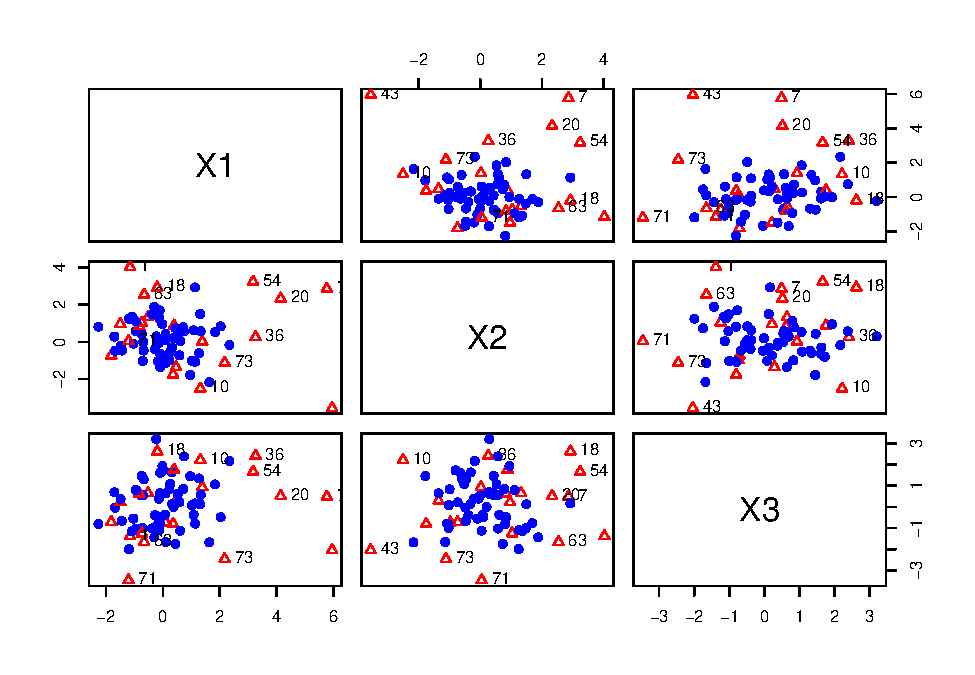
\includegraphics{DifferentVarInflationFactors_files/figure-latex/plotA_training-1.pdf}

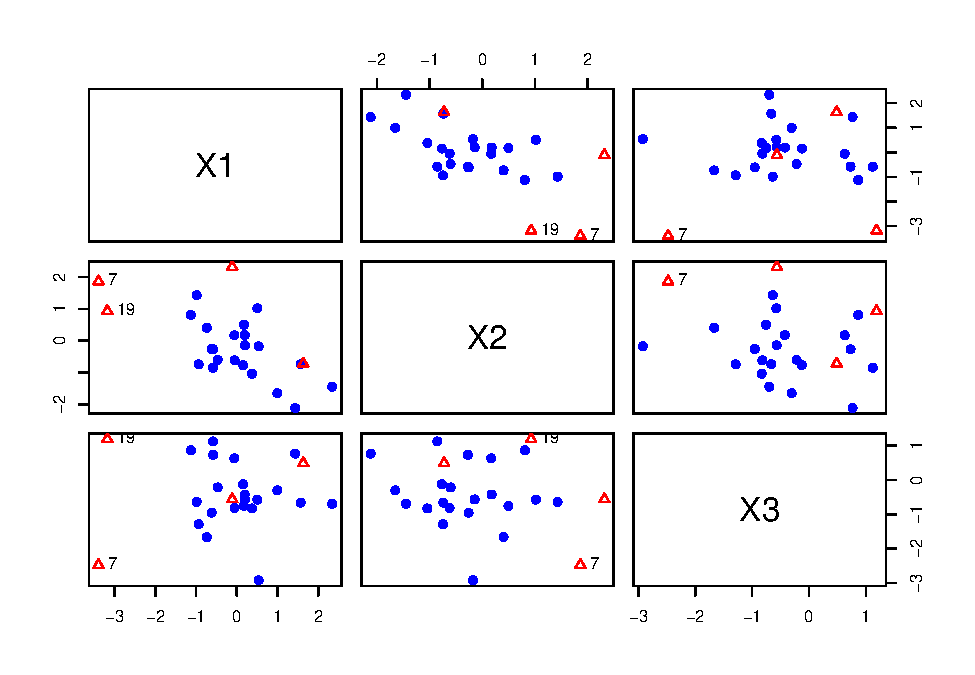
\includegraphics{DifferentVarInflationFactors_files/figure-latex/plotA_test-1.pdf}

Looking at the training data above, it is clear that the inflation
factor is the same across all variables with a few contaminated samples
further than the contaminated samples cloud. This dataset is fitted
firstly with the contaminated mixture of normals model assuming equal
variable inflation factor within group and secondly with the model
assuming different variable inflation factor within group.

\hypertarget{fitting-a-model-with-same-variable-inflation-factor-within-group-for-dataset-a.}{%
\subsubsection{Fitting a model with same variable inflation factor
within group for dataset
A.}\label{fitting-a-model-with-same-variable-inflation-factor-within-group-for-dataset-a.}}

The parameter estimates were obtained by using the command Cnmixt until
covergence from the library ContaminatedMixt. Next, the self-coded
E-step was used to obtain the labels whether a sample is
non-contaminated or contaminated. The function Cnmixt assumes equal
variable inflation factor within group and their estimated parameters
are shown below.

\[
\mu = \begin{bmatrix}-0.01 \\-0.05 \\0.01 \\\end{bmatrix} , \Sigma = \begin{bmatrix}2.41&0&0 \\0&2.41&0 \\0&0&2.41 \\\end{bmatrix}, \alpha = 0.86 , \eta = 4.98
\]

\begin{longtable}[]{@{}lrr@{}}
\caption{Equal IF Train}\tabularnewline
\toprule\noalign{}
& Cont & Non-cont \\
\midrule\noalign{}
\endfirsthead
\toprule\noalign{}
& Cont & Non-cont \\
\midrule\noalign{}
\endhead
\bottomrule\noalign{}
\endlastfoot
Cont & 17 & 23 \\
Non-cont & 0 & 185 \\
\end{longtable}

\begin{longtable}[]{@{}lrr@{}}
\caption{Equal IF Test}\tabularnewline
\toprule\noalign{}
& Cont & Non-cont \\
\midrule\noalign{}
\endfirsthead
\toprule\noalign{}
& Cont & Non-cont \\
\midrule\noalign{}
\endhead
\bottomrule\noalign{}
\endlastfoot
Cont & 11 & 9 \\
Non-cont & 0 & 55 \\
\end{longtable}

\hypertarget{fitting-a-model-with-different-variables-inflation-factor-within-group-using-the-real-parameters-as-initial-values-and-running-an-e-step-to-predict-nu-values-for-dataset-a.}{%
\subsubsection{\texorpdfstring{Fitting a model with different variables
inflation factor within group using the real parameters as initial
values and running an e-step to predict \(\nu\) values for dataset
A.}{Fitting a model with different variables inflation factor within group using the real parameters as initial values and running an e-step to predict \textbackslash nu values for dataset A.}}\label{fitting-a-model-with-different-variables-inflation-factor-within-group-using-the-real-parameters-as-initial-values-and-running-an-e-step-to-predict-nu-values-for-dataset-a.}}

It is assumed the real parameter estimates are known and they are
plug-in the self-coded E-step function to predict samples contamination
in both training and test sets. The confusion matrix where the rows are
the real values and the columns are the predicted ones shows that
42\(\%\), and 55\(\%\) of the contaminated samples are correctly
identified in the training and test set respectively.

\begin{longtable}[]{@{}lrr@{}}
\caption{Train set}\tabularnewline
\toprule\noalign{}
& Cont & Non-cont \\
\midrule\noalign{}
\endfirsthead
\toprule\noalign{}
& Cont & Non-cont \\
\midrule\noalign{}
\endhead
\bottomrule\noalign{}
\endlastfoot
Cont & 21 & 19 \\
Non-cont & 2 & 183 \\
\end{longtable}

\begin{longtable}[]{@{}lrr@{}}
\caption{Test set}\tabularnewline
\toprule\noalign{}
& Cont & Non-cont \\
\midrule\noalign{}
\endfirsthead
\toprule\noalign{}
& Cont & Non-cont \\
\midrule\noalign{}
\endhead
\bottomrule\noalign{}
\endlastfoot
Cont & 11 & 9 \\
Non-cont & 0 & 55 \\
\end{longtable}

\begin{longtable}[]{@{}lrr@{}}
\caption{Train}\tabularnewline
\toprule\noalign{}
Metric & Equal\_IF & Different\_IF \\
\midrule\noalign{}
\endfirsthead
\toprule\noalign{}
Metric & Equal\_IF & Different\_IF \\
\midrule\noalign{}
\endhead
\bottomrule\noalign{}
\endlastfoot
Accuracy & 0.90 & 0.91 \\
Precision & 1.00 & 0.91 \\
Recall & 0.42 & 0.52 \\
Sensitivity & 0.42 & 0.52 \\
Specificity & 1.00 & 0.99 \\
F1 score & 0.60 & 0.67 \\
\end{longtable}

\begin{longtable}[]{@{}lrr@{}}
\caption{Test}\tabularnewline
\toprule\noalign{}
Metric & Equal\_IF & Different\_IF \\
\midrule\noalign{}
\endfirsthead
\toprule\noalign{}
Metric & Equal\_IF & Different\_IF \\
\midrule\noalign{}
\endhead
\bottomrule\noalign{}
\endlastfoot
Accuracy & 0.88 & 0.88 \\
Precision & 1.00 & 1.00 \\
Recall & 0.55 & 0.55 \\
Sensitivity & 0.55 & 0.55 \\
Specificity & 1.00 & 1.00 \\
F1 score & 0.71 & 0.71 \\
\end{longtable}

\hypertarget{using-the-real-contamination-information-nus-and-running-m-step-for-a-model-allowing-different-variable-inflation-factor-within-group-to-obtain-parameter-estimates-for-dataset-a.}{%
\subsubsection{\texorpdfstring{Using the real contamination information
\(\nu\)'s and running m-step for a model allowing different variable
inflation factor within group to obtain parameter estimates for dataset
A.}{Using the real contamination information \textbackslash nu's and running m-step for a model allowing different variable inflation factor within group to obtain parameter estimates for dataset A.}}\label{using-the-real-contamination-information-nus-and-running-m-step-for-a-model-allowing-different-variable-inflation-factor-within-group-to-obtain-parameter-estimates-for-dataset-a.}}

The parameter estimates obtained by using the real contamination
information are

\[
\mu = \begin{bmatrix}-0.05 \\-0.06 \\0.03 \\\end{bmatrix} , \Sigma = \begin{bmatrix}2.77&-0.25&0.14 \\-0.25&0.88&0.1 \\0.14&0.1&3.11 \\\end{bmatrix} , \alpha = 0.82, \dot{N} * \dot{N}^{T} = N = \begin{bmatrix}4.4&0&0 \\0&5.43&0 \\0&0&4.71 \\\end{bmatrix}
\]

\hypertarget{fitting-a-model-with-different-variable-inflation-factor-within-group-using-the-one-obtained-in-an-equal-variable-inflation-factor-within-group-model-as-initial-parameters-for-dataset-a.}{%
\subsubsection{Fitting a model with different variable inflation factor
within group using the one obtained in an equal variable inflation
factor within group model as initial parameters for dataset
A.}\label{fitting-a-model-with-different-variable-inflation-factor-within-group-using-the-one-obtained-in-an-equal-variable-inflation-factor-within-group-model-as-initial-parameters-for-dataset-a.}}

The initial values for the parameters of the model were taken from the
contaminated mixture model produced by the function Cnmixt from the
ContaminatedMixt package that assumes same variable inflation factor
within group. Next, the E-M algorithm with a self-coded m-step that
assumes different variable inflation factor within group for EII model
is run until convergence that was reached after 22 steps. The estimated
parameters are shown below.

\[
\mu = \begin{bmatrix}0.02 \\-0.05 \\-0.09 \\\end{bmatrix} , \Sigma = \begin{bmatrix}3.82&-0.37&0.33 \\-0.37&1.17&0.15 \\0.33&0.15&3.7 \\\end{bmatrix} , \alpha = 0.96, \dot{N} * \dot{N}^{T} = N = \begin{bmatrix}4.62&0&0 \\0&9.05&0 \\0&0&11.32 \\\end{bmatrix}
\]

It is possible to see that there are some differences between the
estimates obtained for both models. The main difference between the
estimates is observed in the values that the model with different
variables inflation factor take for \(\alpha\) which suggest a 0.96 of
non-contaminated samples and implies a greater contamination that the
equal variable inflation factor model 0.86. Also, the inflation factors
in the diagonal of the matrix \(\dot{N}\) are different and much bigger
than the estimated by the equal inflation factor model 5.

It can be seen that the estimate for \(\alpha\) is far from to the true
parameter value. Moreover, the estimates for \(\eta\) assuming different
inflation factor are all different from the true parameter value that is
5. Also, it is possible to see in the diagonal of matrix \(N\) that
\(X_{1}\) and \(X_{2}\) are the variables with inflation factors further
from the true value, while \(X_{3}\) is closer to the true value.

Next, a self-coded function E-step was used to obtain the estimates of
labels corresponding whether the observations are non-contaminated or
contaminated in the test set. It was observed that the estimates for
\(\alpha\) and \(N\) were affected for the choose of the initial values
of \(\nu_{i}\) which denotes if the \(i^{th}\) sample is
non-contaminated if \(\nu_{i}=1\) otherwise is \(0\). The pairs plot of
the samples in the test subset shows a little more dispersion for the
pair \(X_{2}\) and \(X_{3}\) than for the pair \(X_{1}\) and \(X_{3}\).

\begin{longtable}[]{@{}lrr@{}}
\caption{Different IF Train}\tabularnewline
\toprule\noalign{}
& Cont & Non-cont \\
\midrule\noalign{}
\endfirsthead
\toprule\noalign{}
& Cont & Non-cont \\
\midrule\noalign{}
\endhead
\bottomrule\noalign{}
\endlastfoot
Cont & 8 & 32 \\
Non-cont & 0 & 185 \\
\end{longtable}

\begin{longtable}[]{@{}lrr@{}}
\caption{Different IF Test}\tabularnewline
\toprule\noalign{}
& Cont & Non-cont \\
\midrule\noalign{}
\endfirsthead
\toprule\noalign{}
& Cont & Non-cont \\
\midrule\noalign{}
\endhead
\bottomrule\noalign{}
\endlastfoot
Cont & 4 & 16 \\
Non-cont & 0 & 55 \\
\end{longtable}

\hypertarget{comparison-between-model-that-assume-equal-variable-and-different-variable-inflation-factor-within-group-for-dataset-a.}{%
\subsubsection{Comparison between model that assume equal variable and
different variable inflation factor within group for dataset
A.}\label{comparison-between-model-that-assume-equal-variable-and-different-variable-inflation-factor-within-group-for-dataset-a.}}

The confusion matrix where the rows are the actual values and the
columns the predicted values for the model assuming same variable
inflation factor within group , shows that it was possible to identify
half of the contaminated observations and all the non-contaminated
observations correctly.

However, taking a look of the performance of the model assuming
different variables inflation factor within group is also able to
identify half of the non-contaminated samples and misclassified \(3\)
non-contaminated samples as contaminated. As the data is generated for a
model with same variable inflation factor within group, there is not
surprise that it overcame their counterpart that assume different
variable inflation factors within group. It is possible to confirm this
result taking a look to the other metrics specially F1\_Score.

\begin{longtable}[]{@{}lrr@{}}
\caption{Train}\tabularnewline
\toprule\noalign{}
Metric & Equal\_IF & Different\_IF \\
\midrule\noalign{}
\endfirsthead
\toprule\noalign{}
Metric & Equal\_IF & Different\_IF \\
\midrule\noalign{}
\endhead
\bottomrule\noalign{}
\endlastfoot
Accuracy & 0.90 & 0.86 \\
Precision & 1.00 & 1.00 \\
Recall & 0.42 & 0.20 \\
Sensitivity & 0.42 & 0.20 \\
Specificity & 1.00 & 1.00 \\
F1 score & 0.60 & 0.33 \\
\end{longtable}

\begin{longtable}[]{@{}lrr@{}}
\caption{Test}\tabularnewline
\toprule\noalign{}
Metric & Equal\_IF & Different\_IF \\
\midrule\noalign{}
\endfirsthead
\toprule\noalign{}
Metric & Equal\_IF & Different\_IF \\
\midrule\noalign{}
\endhead
\bottomrule\noalign{}
\endlastfoot
Accuracy & 0.88 & 0.79 \\
Precision & 1.00 & 1.00 \\
Recall & 0.55 & 0.20 \\
Sensitivity & 0.55 & 0.20 \\
Specificity & 1.00 & 1.00 \\
F1 score & 0.71 & 0.33 \\
\end{longtable}

\hypertarget{dataset-b}{%
\subsubsection{Dataset B}\label{dataset-b}}

The parameters for dataset B are

\[
\mu = \begin{bmatrix}0 \\0 \\0 \\\end{bmatrix} , \Sigma = I_{3} = \begin{bmatrix}2&0&0 \\0&5&0 \\0&0&7 \\\end{bmatrix}, \alpha = 0.7, \dot{N}_{g} = \begin{bmatrix}1&0&0 \\0&25&0 \\0&0&1 \\\end{bmatrix}, {N}_{g} = \begin{bmatrix}1&0&0 \\0&5&0 \\0&0&1 \\\end{bmatrix}
\] The main different between the second dataset versus the previous one
is that the data is generated from allowing different variables
inflation factor within the group. It is possible to see that \(X_{2}\)
has an inflation factor higher than \(X_{1}\) and \(X_{3}\). The
experiment consist of fitting first the variable assuming the same
variable inflation factor in the group and next allowing different
variable inflation factor within the group and comparing the results
obtained.

{●} True positive (true contaminated predicted as contaminated) {▲} True
negative (true non-contaminated predicted as non-contaminated) {+} False
positive (true non-contaminated predicted as contaminated) {X} False
negative (true contaminated predicted as non-contaminated)

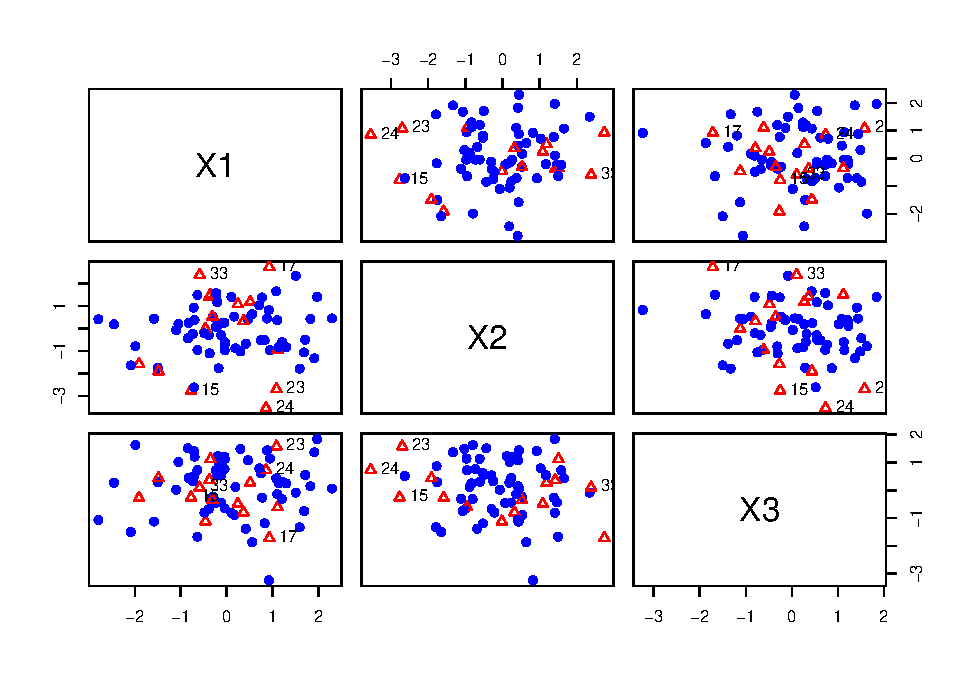
\includegraphics{DifferentVarInflationFactors_files/figure-latex/plotB_training-1.pdf}
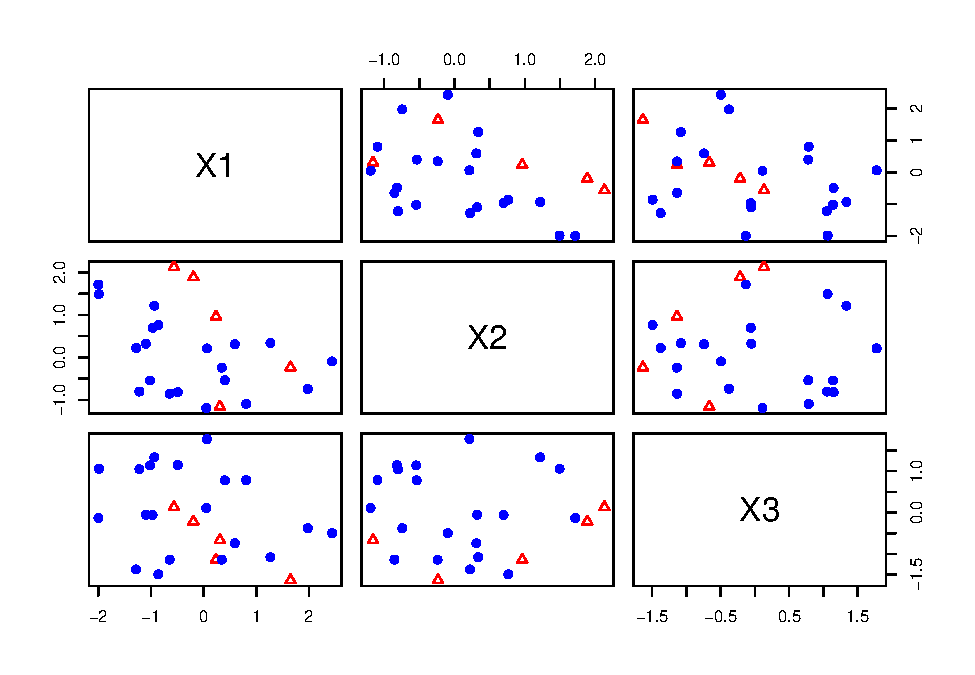
\includegraphics{DifferentVarInflationFactors_files/figure-latex/plotB_test-1.pdf}

It is possible to observe that in the training and test subset there is
a much higher dispersion in the variable \(X2\) with values from \(-10\)
to \(8\) in comparison with \(X_{1}\) and \(X_{3}\).

\hypertarget{fitting-a-model-with-same-variable-inflation-factor-within-group-for-dataset-b.}{%
\subsubsection{Fitting a model with same variable inflation factor
within group for dataset
B.}\label{fitting-a-model-with-same-variable-inflation-factor-within-group-for-dataset-b.}}

Similar procedure is carry out fitting the data using Cnmixt function
for model EII and assuming same variable inflation factor in the group
and the parameters obtained are:

\[
\mu = \begin{bmatrix}0.03 \\0.09 \\-0.05 \\\end{bmatrix} , \Sigma = \begin{bmatrix}5.06&0&0 \\0&5.06&0 \\0&0&5.06 \\\end{bmatrix}, \alpha = 0.83 , \eta = 12.29
\]

\begin{longtable}[]{@{}lrr@{}}
\caption{Equal IF Train}\tabularnewline
\toprule\noalign{}
& Cont & Non-cont \\
\midrule\noalign{}
\endfirsthead
\toprule\noalign{}
& Cont & Non-cont \\
\midrule\noalign{}
\endhead
\bottomrule\noalign{}
\endlastfoot
Cont & 247 & 281 \\
Non-cont & 18 & 1254 \\
\end{longtable}

\begin{longtable}[]{@{}lrr@{}}
\caption{Equal IF Test}\tabularnewline
\toprule\noalign{}
& Cont & Non-cont \\
\midrule\noalign{}
\endfirsthead
\toprule\noalign{}
& Cont & Non-cont \\
\midrule\noalign{}
\endhead
\bottomrule\noalign{}
\endlastfoot
Cont & 195 & 174 \\
Non-cont & 10 & 821 \\
\end{longtable}

\hypertarget{fitting-a-model-with-different-variables-inflation-factor-within-group-using-the-real-parameters-as-initial-values-and-running-an-e-step-to-predict-nu-values-for-dataset-b.}{%
\subsubsection{\texorpdfstring{Fitting a model with different variables
inflation factor within group using the real parameters as initial
values and running an e-step to predict \(\nu\) values for dataset
B.}{Fitting a model with different variables inflation factor within group using the real parameters as initial values and running an e-step to predict \textbackslash nu values for dataset B.}}\label{fitting-a-model-with-different-variables-inflation-factor-within-group-using-the-real-parameters-as-initial-values-and-running-an-e-step-to-predict-nu-values-for-dataset-b.}}

It is assumed that the real parameters are known and they are used as an
input for a self-coded E-step as it was done previously to produce
estimates for \(\nu\)'s. From the tables below it is possible to see
that half of the contaminated samples and any of them were identified in
the train and test subsets respectively.

\begin{longtable}[]{@{}lrr@{}}
\toprule\noalign{}
& Cont & Non-cont \\
\midrule\noalign{}
\endhead
\bottomrule\noalign{}
\endlastfoot
Cont & 320 & 208 \\
Non-cont & 33 & 1239 \\
\end{longtable}

\begin{longtable}[]{@{}lrr@{}}
\toprule\noalign{}
& Cont & Non-cont \\
\midrule\noalign{}
\endhead
\bottomrule\noalign{}
\endlastfoot
Cont & 242 & 127 \\
Non-cont & 21 & 810 \\
\end{longtable}

\begin{longtable}[]{@{}lrr@{}}
\caption{Metrics train set}\tabularnewline
\toprule\noalign{}
Metric & Equal\_IF & Different\_IF \\
\midrule\noalign{}
\endfirsthead
\toprule\noalign{}
Metric & Equal\_IF & Different\_IF \\
\midrule\noalign{}
\endhead
\bottomrule\noalign{}
\endlastfoot
Accuracy & 0.83 & 0.87 \\
Precision & 0.93 & 0.91 \\
Recall & 0.47 & 0.61 \\
Sensitivity & 0.47 & 0.61 \\
Specificity & 0.99 & 0.97 \\
F1 score & 0.62 & 0.73 \\
\end{longtable}

\begin{longtable}[]{@{}lrr@{}}
\caption{Metrics test set}\tabularnewline
\toprule\noalign{}
Metric & Equal\_IF & Different\_IF \\
\midrule\noalign{}
\endfirsthead
\toprule\noalign{}
Metric & Equal\_IF & Different\_IF \\
\midrule\noalign{}
\endhead
\bottomrule\noalign{}
\endlastfoot
Accuracy & 0.85 & 0.88 \\
Precision & 0.95 & 0.92 \\
Recall & 0.53 & 0.66 \\
Sensitivity & 0.53 & 0.66 \\
Specificity & 0.99 & 0.97 \\
F1 score & 0.68 & 0.77 \\
\end{longtable}

\hypertarget{using-the-real-contamination-information-nus-to-run-a-m-step-for-a-model-allowing-different-variable-inflation-factor-within-group-to-obtain-parameter-estimates-for-dataset-b.}{%
\subsubsection{\texorpdfstring{Using the real contamination information
\(\nu\)'s to run a m-step for a model allowing different variable
inflation factor within group to obtain parameter estimates for dataset
B.}{Using the real contamination information \textbackslash nu's to run a m-step for a model allowing different variable inflation factor within group to obtain parameter estimates for dataset B.}}\label{using-the-real-contamination-information-nus-to-run-a-m-step-for-a-model-allowing-different-variable-inflation-factor-within-group-to-obtain-parameter-estimates-for-dataset-b.}}

The parameter estimates for \(\mu,\Sigma\) are quite close to the true
parameter values. The model to be fitted has covariance structure (VVV).
There is a noticeable different in the estimate for \(\alpha\) with
respect to its true value. The estimation for \(\alpha\) assumes that
there are more contaminated samples than what the true parameter states.
The estimation for \(\eta\) for each variable is visible in the diagonal
of the matrix \(N\). The model reaches convergence after 25 steps and
the parameter estimates are:

\[
\mu = \begin{bmatrix}0.03 \\0.05 \\-0.03 \\\end{bmatrix} , \Sigma = \begin{bmatrix}1.98&0.03&-0.01 \\0.03&4.91&0.12 \\-0.01&0.12&6.85 \\\end{bmatrix} , \alpha = 0.71, \dot{N} * \dot{N}^{T} = N = \begin{bmatrix}1&0&0 \\0&22.28&0 \\0&0&1 \\\end{bmatrix}
\]

\hypertarget{fitting-a-model-with-different-variable-inflation-factor-within-group-using-the-one-obtained-in-an-equal-variable-inflation-factor-within-group-model-as-initial-parameters-for-dataset-b.}{%
\subsubsection{Fitting a model with different variable inflation factor
within group using the one obtained in an equal variable inflation
factor within group model as initial parameters for dataset
B.}\label{fitting-a-model-with-different-variable-inflation-factor-within-group-using-the-one-obtained-in-an-equal-variable-inflation-factor-within-group-model-as-initial-parameters-for-dataset-b.}}

The parameters obtained for \(\mu\), and \(\Sigma\) are very similar to
their true values. The main difference between the estimates produced by
a model assuming equal variable inflation factors and different variable
inflation factors lies in the estimates for \(\alpha\). For the former
model \(\alpha\) is equal to 0.71 while the latter is equal to 0.89
which means that it overestimated the percentage of non-contaminated
samples. Also, the variable inflation factors estimates are different
for all the variables as the elements of the diagonal of matrix \(N\)
shows. Moreover, the estimate for the variable inflation factor
corresponding to \(X_{2}\) is greater than its true value.

\[
\mu = \begin{bmatrix}0.03 \\0.12 \\-0.03 \\\end{bmatrix} , \Sigma = \begin{bmatrix}1.77&-0.04&-0.05 \\-0.04&9.06&0.09 \\-0.05&0.09&6.04 \\\end{bmatrix} , \alpha = 0.89, \dot{N} * \dot{N}^{T} = N = \begin{bmatrix}1.11&0&0 \\0&27.79&0 \\0&0&1.27 \\\end{bmatrix}
\] Taking a look of the performance of the model assuming same variable
inflation factor within group we can see that it is able to identify 33
and 35 contaminated samples in the training and test sets.

\begin{longtable}[]{@{}lrr@{}}
\caption{Different IF Train}\tabularnewline
\toprule\noalign{}
& Cont & Non-cont \\
\midrule\noalign{}
\endfirsthead
\toprule\noalign{}
& Cont & Non-cont \\
\midrule\noalign{}
\endhead
\bottomrule\noalign{}
\endlastfoot
Cont & 175 & 353 \\
Non-cont & 0 & 1272 \\
\end{longtable}

\begin{longtable}[]{@{}lrr@{}}
\caption{Different IF Test}\tabularnewline
\toprule\noalign{}
& Cont & Non-cont \\
\midrule\noalign{}
\endfirsthead
\toprule\noalign{}
& Cont & Non-cont \\
\midrule\noalign{}
\endhead
\bottomrule\noalign{}
\endlastfoot
Cont & 128 & 241 \\
Non-cont & 0 & 831 \\
\end{longtable}

\hypertarget{comparison-between-model-that-assume-equal-variable-and-different-variable-inflation-factor-within-group-for-dataset-b.}{%
\subsubsection{Comparison between model that assume equal variable and
different variable inflation factor within group for dataset
B.}\label{comparison-between-model-that-assume-equal-variable-and-different-variable-inflation-factor-within-group-for-dataset-b.}}

The rest of the metrics confirms that when the data was coming from
different variables inflation factors the model allowing different
inflation factor seems to be more appropriate than assuming equal
inflation factor within group as long as the initial parameters values
are close to the true values.

\begin{longtable}[]{@{}lrr@{}}
\caption{Train}\tabularnewline
\toprule\noalign{}
Metric & Equal\_IF & Different\_IF \\
\midrule\noalign{}
\endfirsthead
\toprule\noalign{}
Metric & Equal\_IF & Different\_IF \\
\midrule\noalign{}
\endhead
\bottomrule\noalign{}
\endlastfoot
Accuracy & 0.83 & 0.80 \\
Precision & 0.93 & 1.00 \\
Recall & 0.47 & 0.33 \\
Sensitivity & 0.47 & 0.33 \\
Specificity & 0.99 & 1.00 \\
F1 score & 0.62 & 0.50 \\
\end{longtable}

\begin{longtable}[]{@{}lrr@{}}
\caption{Test}\tabularnewline
\toprule\noalign{}
Metric & Equal\_IF & Different\_IF \\
\midrule\noalign{}
\endfirsthead
\toprule\noalign{}
Metric & Equal\_IF & Different\_IF \\
\midrule\noalign{}
\endhead
\bottomrule\noalign{}
\endlastfoot
Accuracy & 0.85 & 0.80 \\
Precision & 0.95 & 1.00 \\
Recall & 0.53 & 0.35 \\
Sensitivity & 0.53 & 0.35 \\
Specificity & 0.99 & 1.00 \\
F1 score & 0.68 & 0.52 \\
\end{longtable}

\end{document}
